\textit{Come faccio a fare le cose?}\newline
Asse realizzato molto bene, con qualche piccola pecca. Sono presenti:
\begin{itemize}
	\item \textbf{Menu:} Verrà trattato meglio in \fullref{sec:BarraDiNavigazione}. Bene il posizionamento, meno bene alcune voci del menù, come \textit{"Spazi che parlano di te"} che costringono l'utente a fare \textit{click gambling} per scoprire cosa fanno.
	\item \textbf{Barra di ricerca:} Presente in alto a destra tramite il simbolo della lente di ingrandimento. Bene.
	\item \textbf{Link:} Sono presenti paragrafi con link e immagini cliccabili che rimandano alle sezioni del sito. Male però la non cliccabilità dei titoli del paragrafo. La funzione di link è delegata a un collegamento che potrebbe essere rimosso (\autoref{fig:LinkInutile}).
	\item \textbf{Chat live:} Presente in basso a destra, permette di chiedere informazioni live via chat a un persona vera. La chat rimane aperta anche durante la navigazione in altre pagine e presenta un sforzo computazionale per l'utente decisamente inferiore a quello di una chiamata. Bene.
\end{itemize}

\begin{figure}
	\centering
	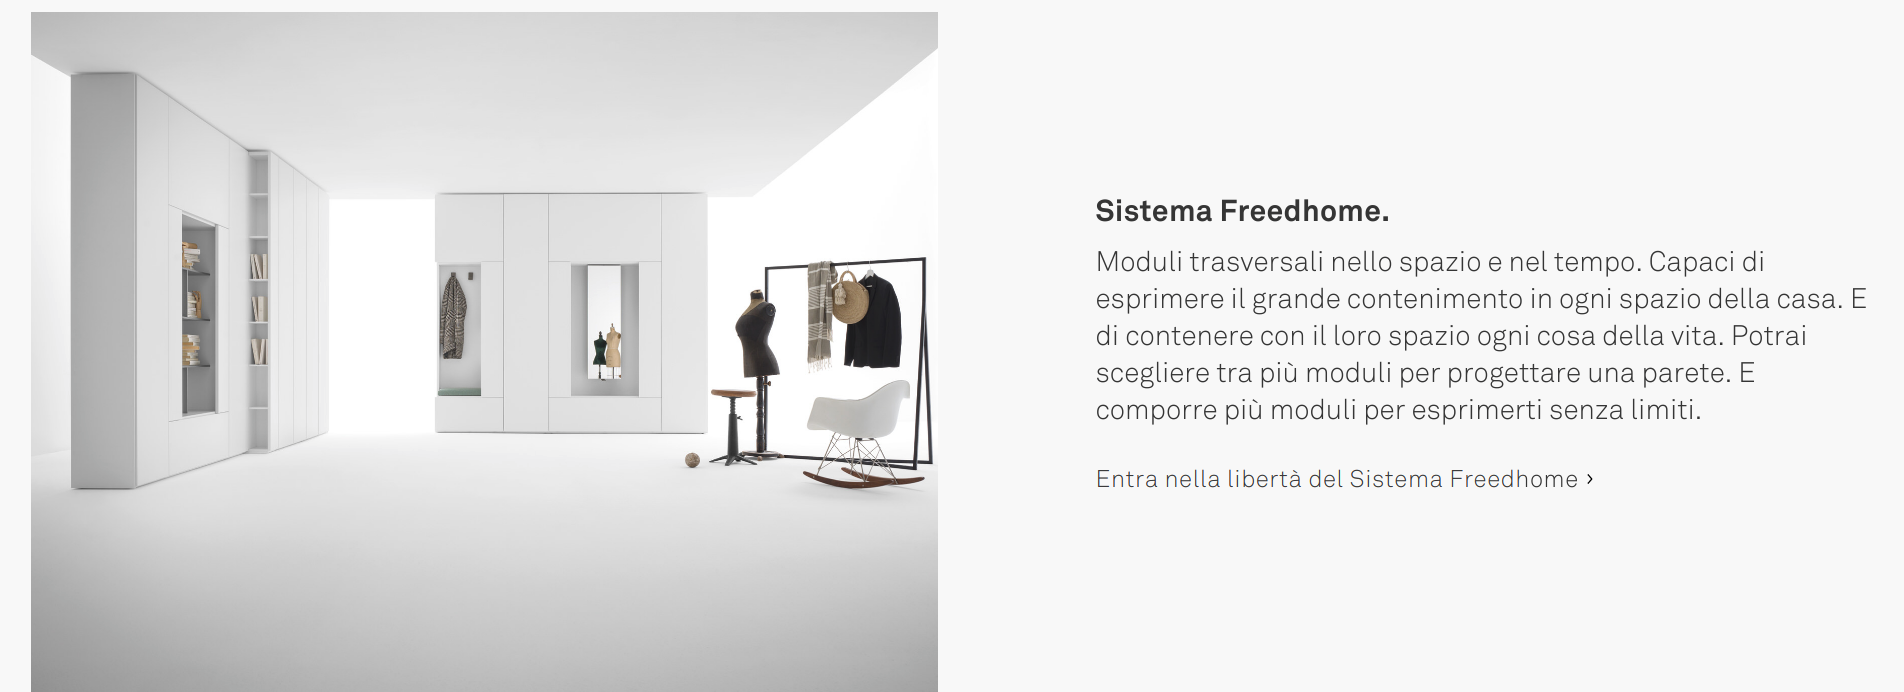
\includegraphics[width=\textwidth]{sez/HomePage/img/Link.png}
	\caption[https://www.caccaro.com/]{Clicca qui per... Sarebbe stato meglio rendere cliccabile il titolo del paragrafo}
	\label{fig:LinkInutile}
\end{figure}